%%%%%%%%%%%%%%%%%%%%%%%%%%%%%%%%%%%%%%%%%
% Beamer Presentation
% LaTeX Template
% Version 1.0 (10/11/12)
%
% This template has been downloaded from:
% http://www.LaTeXTemplates.com
%
% License:
% CC BY-NC-SA 3.0 (http://creativecommons.org/licenses/by-nc-sa/3.0/)
%
%%%%%%%%%%%%%%%%%%%%%%%%%%%%%%%%%%%%%%%%%

%----------------------------------------------------------------------------------------
%	PACKAGES AND THEMES
%----------------------------------------------------------------------------------------

\documentclass{beamer}

\mode<presentation> {
	
	% The Beamer class comes with a number of default slide themes
	% which change the colors and layouts of slides. Below this is a list
	% of all the themes, uncomment each in turn to see what they look like.
	
	%\usetheme{default}
	%\usetheme{AnnArbor}
	%\usetheme{Antibes}
	%\usetheme{Bergen}
	%\usetheme{Berkeley}
	%\usetheme{Berlin}
	%\usetheme{Boadilla}
	%\usetheme{CambridgeUS}
	%\usetheme{Copenhagen}
	%\usetheme{Darmstadt}
	%\usetheme{Dresden}
	%\usetheme{Frankfurt}
	%\usetheme{Goettingen}
	%\usetheme{Hannover}
	%\usetheme{Ilmenau}
	%\usetheme{JuanLesPins}
	%\usetheme{Luebeck}
	\usetheme{Madrid}
	%\usetheme{Malmoe}
	%\usetheme{Marburg}
	%\usetheme{Montpellier}
	%\usetheme{PaloAlto}
	%\usetheme{Pittsburgh}
	%\usetheme{Rochester}
	%\usetheme{Singapore}
	%\usetheme{Szeged}
	%\usetheme{Warsaw}
	
	% As well as themes, the Beamer class has a number of color themes
	% for any slide theme. Uncomment each of these in turn to see how it
	% changes the colors of your current slide theme.
	
	%\usecolortheme{albatross}
	%\usecolortheme{beaver}
	%\usecolortheme{beetle}
	%\usecolortheme{crane}
	%\usecolortheme{dolphin}
	%\usecolortheme{dove}
	%\usecolortheme{fly}
	%\usecolortheme{lily}
	%\usecolortheme{orchid}
	\usecolortheme{rose}
	%\usecolortheme{seagull}
	%\usecolortheme{seahorse}
	%\usecolortheme{whale}
	%\usecolortheme{wolverine}
	
	%\setbeamertemplate{footline} % To remove the footer line in all slides uncomment this line
	%\setbeamertemplate{footline}[page number] % To replace the footer line in all slides with a simple slide count uncomment this line
	
	\setbeamertemplate{navigation symbols}{} % To remove the navigation symbols from the bottom of all slides uncomment this line
}

\usepackage{graphicx} % Allows including images
\usepackage{booktabs} % Allows the use of \toprule, \midrule and \bottomrule in tables
\usepackage{inputenc}
%----------------------------------------------------------------------------------------
%	TITLE PAGE
%----------------------------------------------------------------------------------------

\title[Intro to FOSS]{Introduction to FOSS} % The short title appears at the bottom of every slide, the full title is only on the title page

\author{\color{cyan}{Software Freedom Day}} % Your name
\institute[AITI-GI-KACE] % Your institution as it will appear on the bottom of every slide, may be shorthand to save space
{
	GHANA-INDIA KOFI ANNAN CENTER OF EXCELLENCE IN INFORMATION TECHNOLOGY \\
	(ADVANCED INFORMATION TECHONOLOGY INSTITUTE) \\ % Your institution for the title page
	\medskip
	\textit{\textbf{aiti-kace.com.gh}} % Your email address
}
\date{\today} % Date, can be changed to a custom date

\begin{document}
	
	\begin{frame}
		\titlepage % Print the title page as the first slide
	\end{frame}
	
	\begin{frame}
		\frametitle{Overview} % Table of contents slide, comment this block out to remove it
		\tableofcontents % Throughout your presentation, if you choose to use \section{} and \subsection{} commands, these will automatically be printed on this slide as an overview of your presentation
	\end{frame}
	
	%----------------------------------------------------------------------------------------
	%	PRESENTATION SLIDES
	%----------------------------------------------------------------------------------------
	
	%------------------------------------------------
	\begin{frame}
	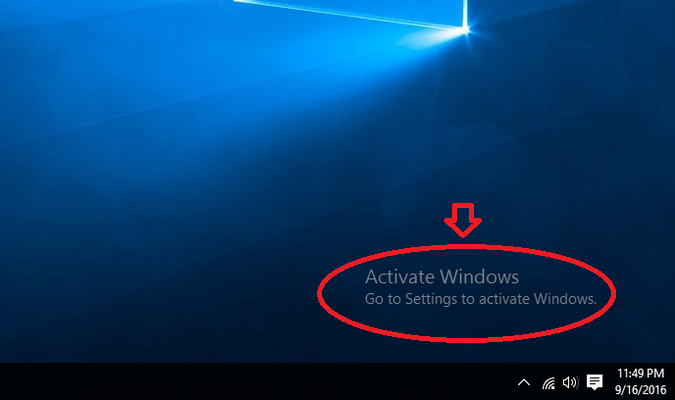
\includegraphics[width=0.6\linewidth]{activatewatermark}
	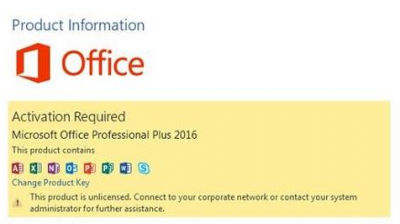
\includegraphics[width=0.6\linewidth]{activateoffice.png}
	\end{frame}


	\section{What is FOSS?} 
	%------------------------------------------------
	\begin{frame}\frametitle{What is FOSS?}
		\color{cyan}{\textbf{\textit{\underline{F}}}ree and \textbf{\textit{\underline{O}}}pen \textbf{\textit{\underline{S}}}ource \textbf{\textit{\underline{S}}}oftware ==
		FOSS}
		\begin{figure}
			
\includegraphics[scale =0.6]{sfoss}
		\end{figure}
	\end{frame}
	\begin{frame} \frametitle{Source code vs Executable}
	\begin{figure}
		\begin{center}
			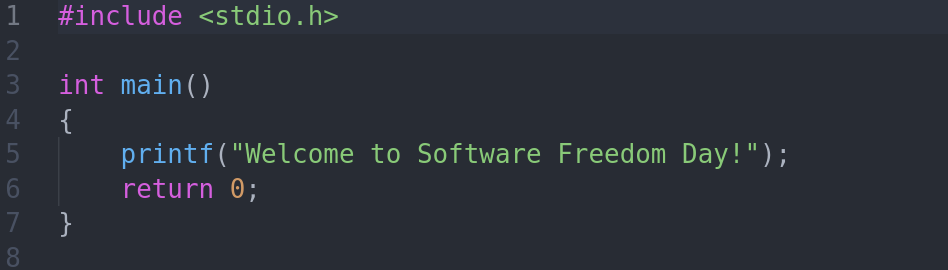
\includegraphics[width=0.5\linewidth]{welcomec.png}
			\caption{1.Source code}
		\end{center}
		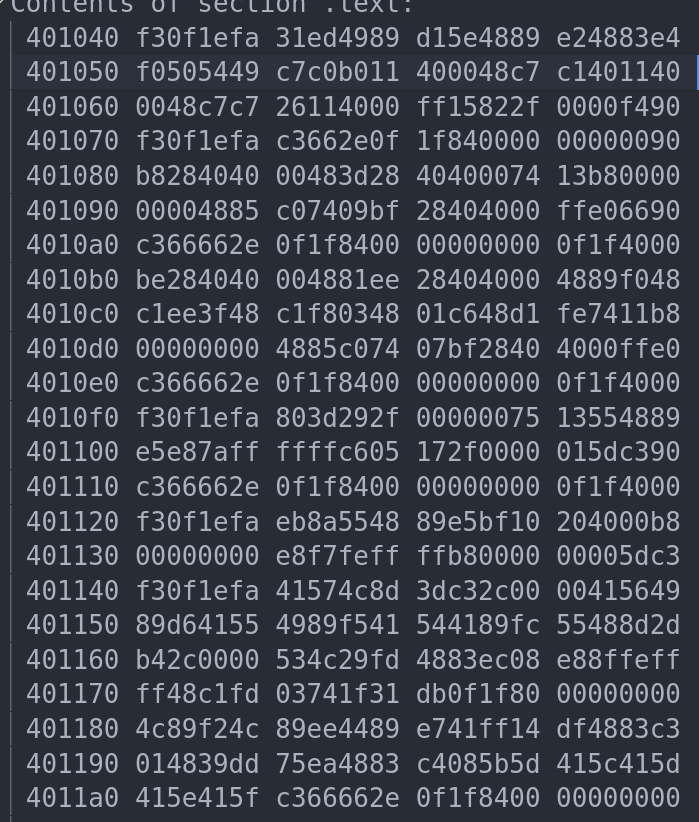
\includegraphics[width=0.3\linewidth]{welcomeobj.png}
		\caption{2.Executable}
	\end{figure}
\end{frame}

%	\subsection{Brief History} 
%	\begin{frame}
%	\frametitle{Brief History}
%	\begin{block}{GNU Project}
%		1983: Richard Stallman started the GNU project \newline
%		1985: Stallman starts Free Software Foundation(FSF)
%	\end{block}
%	\begin{block}{Open Source Software}
%		1998: Netscape releases its source code under Netscape Public License \newline
%		1998: Bruce Perens and Eric S. Raymond start Open Source Initiative (OSI)
%	\end{block}

%\begin{block}{GNU/Linux}
%	1991: Torvalds Linus releases the first version of the Linux Kernel \newline
%	To make an OS, a kernel and other supporting programs are needed
%	\newline \textbf{\textit{Linux}} is the kernel while most of the supporting programs like: \newline Compiler toolchains and user programs are from \textbf{\textit{GNU} and other projects}
%\end{block}
%\end{frame}
	
	\subsection{Free Software}
\begin{frame}
	\frametitle{Free Software}
	\begin{block}{Free Speech, not Free Lunch or Beer}
		Free software does not necessarily imply zero monetary cost \newline
		However, most FOSS comes at no monetary cost to the user.
	\end{block}
	\begin{block}{The Four Essential Freedoms making Software Free}
		\begin{itemize}
			\item {\color{red}{Freedom 0}}: \textit{\textbf{Run}} |the program as you wish, for any purpose 
			\item {\color{red}{Freedom 1}}: \textbf{\textit{Study}} | how the program works, and change it so it does your computing as you wish \newline
			{\color{blue}{\textit{Implies access to source code}}}
			\item {\color{red}{Freedom 2}}: \textbf{\textit{Share }}| redistribute copies so you can help others
			\item {\color{red}{Freedom 3}}: \textbf{\textit{Improve}} | distribute copies of your modified versions to others 
		\end{itemize}
	\end{block}
\end{frame}

\begin{frame}\frametitle{Open Source}
		\begin{block}{Open Source }
			\begin{itemize}
				\item Source code available to user
				\item User able to modify
			\end{itemize}
		\end{block}
\end{frame}

	\subsection{Licenses}
\begin{frame}
	\frametitle{Licenses and Copyright}
	\begin{block}{Copyright}
		\begin{itemize}
			\item Original work of an author is protected from unauthorized use
			\item Original author can do almost anything he wants with his/her work
			\item He/She can sell off the work to others
		\end{itemize}
		
	\end{block}
	
	\begin{block}{Licenses}
		Due to Copyright law, software is non-free by default 
	\end{block}
\end{frame}
\begin{frame} \frametitle{Licenses | GPL}
	\begin{block}{GNU GPL}
		\begin{figure}
			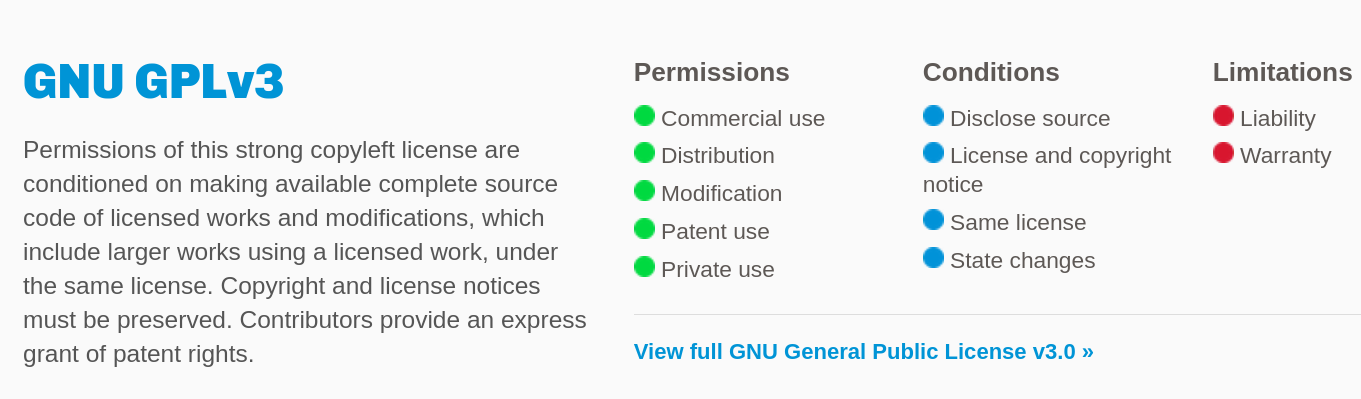
\includegraphics[scale =1]{gpl}
		\end{figure}
	\end{block}
\end{frame}
\begin{frame} \frametitle{Licenses | MIT}
	\begin{block}{MIT}
		\begin{figure}
			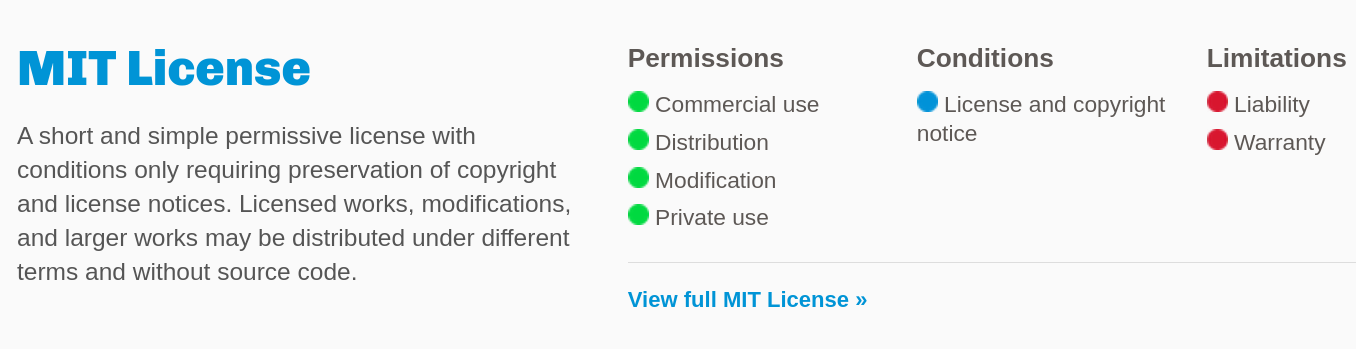
\includegraphics[scale =1]{mit}
		\end{figure}
	\end{block}
\end{frame}


	\subsection{Examples and Sources of FOSS projects }
	\begin{frame}
		\frametitle{Examples of FOSS projects}
		\begin{itemize}
			\item GCC,Codeblocks,VSCode || for devs
			\item OpenOffice,LibreOffice ||for Office productivity
			\item GIMP || for graphics designers
			\item GNU Octave ||for Scientists and Engineers
			\item Thunderbird || a mail client
			\item GNU/Linux OS and the various distributions
			\item The *BSDs
			\item The Android project
			\item Apache Web server
			\item PostgreSQL, MySQL || DBMS
			\item Perl, PHP, Python || Scripting languages
			\item Wordpress || Blogging
		\end{itemize}
	\end{frame}
	\begin{frame}
		\begin{flushleft}
			\begin{figure}
			
\includegraphics[scale =0.9]{dev.png}
		\end{figure}
		\end{flushleft}
	\begin{figure}
		
\includegraphics[scale =0.1]{git.png}
		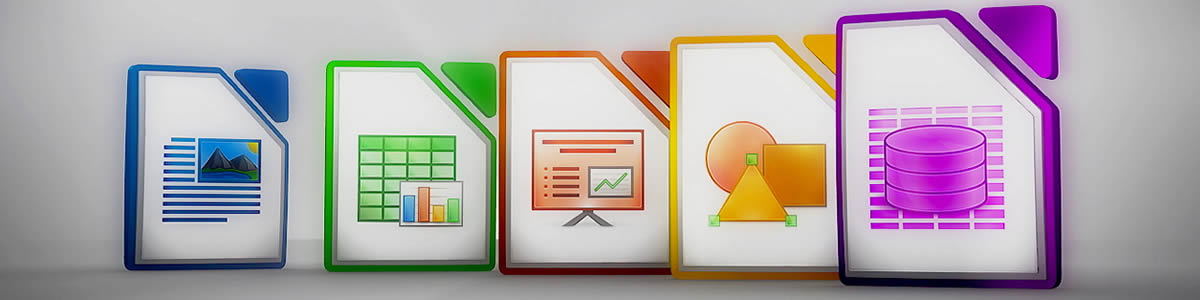
\includegraphics[scale=.1]{openoffice}
	\end{figure}
	\end{frame}
	\begin{frame}
		\frametitle{Sources of FOSS projects}
		\begin{itemize}
			\item gnu.org
			\item github.com | software is provided in source code format
			\item sourceforge.net
			\item framadvd.org
		\end{itemize}
	\end{frame}
	
%	\subsection{FOSS versus Proprietary}
%	\begin{frame}
%		\frametitle{FOSS versus Proprietary}
%		\begin{columns}[c] % The "c" option specifies centered vertical alignment while the "t" option is used for top vertical alignment
			
%			\column{.5\textwidth} % Left column and width
%			\textbf{FOSS}
%			\begin{enumerate}
%				\item Source code is in the public domain \newline
%				\item Software is presented as both source code and executable \newline \newline
%				\item Use is encouraged by FOSS licenses that protect the user \newline \newline
%			\end{enumerate}
			
%			\column{.5\textwidth} % 
%			\textbf{Proprietary}
%			\begin{enumerate}
%				\item Source code is kept from the public \newline
%				\item Software is presented as purely executable | if made available at all, at extra cost to the user \newline
%				\item Use(eg. number of instances run) is restricted by lengthy End User License Agreements \newline
%			\end{enumerate}
%		\end{columns}
		
%	\end{frame}
	%------------------------------------------------
	\section{Why should you care?}
	\begin{frame}{Why should you care?}
		\begin{block}{Cost}
			\begin{itemize}
				\item Usually free
				\item Significantly cheaper than proprietary software
			\end{itemize}
		\end{block}
		\begin{block}{Escape Vendor Lock in}
		\begin{itemize}
			\item Use software from whichever company you are comfortable with
			\item Switch technologies when you wish
		\end{itemize}
	\end{block}
		\begin{block}{Ethical}
			\begin{itemize}
				\item Percentage of softwares in this country are pirated
				\item With FOSS, that figure goes right to Zero percent
				\item Saves firms/users from litigation over permission to do stuff with the bought software
			\end{itemize}
		\end{block}
	\end{frame}
	\begin{frame}{}
		\begin{block}{Legal computing power}
			\begin{itemize}
				\item Anyone can use it without any legal issues
			\end{itemize}
		\end{block}
		\begin{block}{Promotes Education}
			\begin{itemize}
				\item Students interested in such things can peruse the code running on real world systems
				\item Students everywhere can access cutting edge technology
			\end{itemize}
		\end{block}
		\begin{block}{Trust worthy}
			\begin{itemize}
				\item You know what your software does
				\item No hidden agenda
				\item Bugs are easily identified and resolved**
			\end{itemize}
		\end{block}
	\end{frame}
	\subsection{Cost}
	\subsection{Escape vendor lock in}
	\subsection{Ethical}
	%------------------------------------------------


	%------------------------------------------------
	\section{How do you participate?}
	\begin{frame}{How do you participate?}
			\begin{block}{Use}
				\begin{itemize}
					\item It is usually devoid of monetary cost
					\item Significantly cheaper than proprietary software
					\item Tell others too
				\end{itemize}
			\end{block}
			\begin{block}{Report bugs}
				\begin{itemize}
					\item Tell the dev challenges with the current version
					\item Suggest features
				\end{itemize}
			\end{block}
			\begin{block}{Contribute}
				\begin{itemize}
					\item Source code
					\item Write documentation
					\item Translate 
					\item Sponsor
				\end{itemize}
			\end{block}
		\end{frame}
	\subsection{Use}
	\subsection{Report bugs}
	\subsection{Contribute}
	

	%------------------------------------------------
	\begin{frame}{What have we learnt?}
		\begin{block}{What FOSS is.}
			\begin{figure}
				
\includegraphics[scale =0.4]{4freedoms.png}
			\end{figure}
		\end{block}
		\begin{block}{Why you should care.}
		\begin{itemize}
			\item Significantly cheaper than alternatives
			\item Ethical and Legal
			\item Trustworthy
		\end{itemize}
	\end{block}
		\begin{block}{How you can participate.}
		\begin{itemize}
			\item Use FOSS
			\item Report bugs
			\item Contribute
		\end{itemize}
		\end{block}
	\end{frame}

	%------------------------------------------------
	
	\begin{frame}
		\frametitle{References}
		\footnotesize{
		\begin{itemize}
			\item https://choosealicense.com/licenses/
			\item gnu.org
			\item opensource.org
		\end{itemize}
		}
	\end{frame}
	

	%------------------------------------------------
		\begin{frame} \frametitle{Tux says:}
			\begin{figure}
			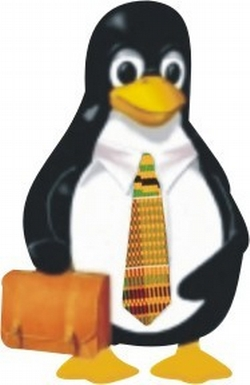
\includegraphics[width = 0.3\linewidth]{ghTux.jpg}
			\textbf{\textit{{\large Tux says:} {\Huge THANK YOU!}}}
			\end{figure}	
		\end{frame}


	
	%----------------------------------------------------------------------------------------
	
\end{document} 